% Section 1 - Introduction
% Roberto Masocco <roberto.masocco@uniroma2.it>
% April 12, 2026

% ### Introduction ###
\section{Introduction}
\graphicspath{{figs/section1/}}

% --- Information ---
\begin{frame}{Information}
  \justifying
	\begin{itemize}
		\item \textbg{Calendar}: from April 22 to June 11, 2026, see Teams for schedule.
		\item \textbg{Topics}:
		      \begin{enumerate}
			      \item Middleware for robotics.
			      \item Basics of C++ programming and version control.
			      \item Development tools for robotics (\emph{e.g.}, Docker).
			      \item Integration of sensors and hardware devices.
			      \item Introduction to localization and mapping (SLAM), autonomous navigation.
			      \item Automata and agents.
			      \item Practical examples.
		      \end{enumerate}
	\end{itemize}
\end{frame}
\begin{frame}{Information}
  \justifying
	\begin{itemize}
		\item \textbg{Materials}:
		      \begin{itemize}
			      \item Code repository: \href{https://github.com/IntelligentSystemsLabUTV/ros2-examples}{\color{blue}\underline{github.com/ros2-examples}} (\texttt{jazzy} branch).
			      \begin{itemize}
              \item Updated regularly, run \texttt{git~pull} before each lecture.
            \end{itemize}
			      \item Lectures: \href{https://github.com/stars/robmasocco/lists/dafn26}{\color{blue}\underline{github.com/robmasocco}}, Teams directory (this lecture is \href{https://github.com/robmasocco/DAFN26_Robotics_1}{\color{blue}\underline{here}}).
			      \item Textbook (if you really really need it): \href{http://dx.doi.org/10.13140/RG.2.2.30948.90247}{\color{blue}\underline{my PhD thesis}}.
		      \end{itemize}
		\item \textbg{Useful background}:
		      \begin{itemize}
			      \item Basics of C and Python programming, everyday Linux commands, and a Unix-like system.
			      \item Basics of Git workflow (check out \href{https://www.atlassian.com/git/tutorials/what-is-git}{\color{blue}\underline{this tutorial}} by Atlassian).
		      \end{itemize}
		\visible<2>{\item \textbg{Exam/thesis}: ... ask Prof. Carnevale \smiley~some projects may be proposed later on.}
	\end{itemize}
\end{frame}

% --- Survey ---
\begin{frame}{Survey}
  \justifying
	Please answer without fear!\\
	\bigskip
	Who knows what about:
	\begin{itemize}
		\visible<2->{\item Version control and Git?}
    \visible<3->{\item Python?}
    \visible<4->{\item C/C++, from coding to linking?}
    \visible<5->{\item Object-Oriented Programming (OOP)?}
    \visible<6->{\item Networking and the ISO/OSI model?}
    \visible<7->{\item Extended Kalman Filter and variants?}
    \visible<8->{\item Finite-State Machines and automata?}
	\end{itemize}
\end{frame}

% --- The roboticist ---
\begin{frame}{The roboticist}{A new path for control engineers}
	\begin{columns}
		\column{.5\textwidth}
    \justifying
		A \textbg{control engineer} is a specialist in the \textbg{design} of controllers to drive \textbg{dynamic systems}; the implementation was traditionally left to other specialists.\\
		A \textbg{roboticist} is a specialist capable of designing, \textbg{building}, and \textbg{programming} complex \textbg{autonomous systems}; with skills ranging from computer science to other disciplines.
		\begin{block}{}
			\centering
			\textbf{A control engineer can be very effective as a roboticist.}
		\end{block}

		\column{.5\textwidth}
		\begin{figure}
			\centering
			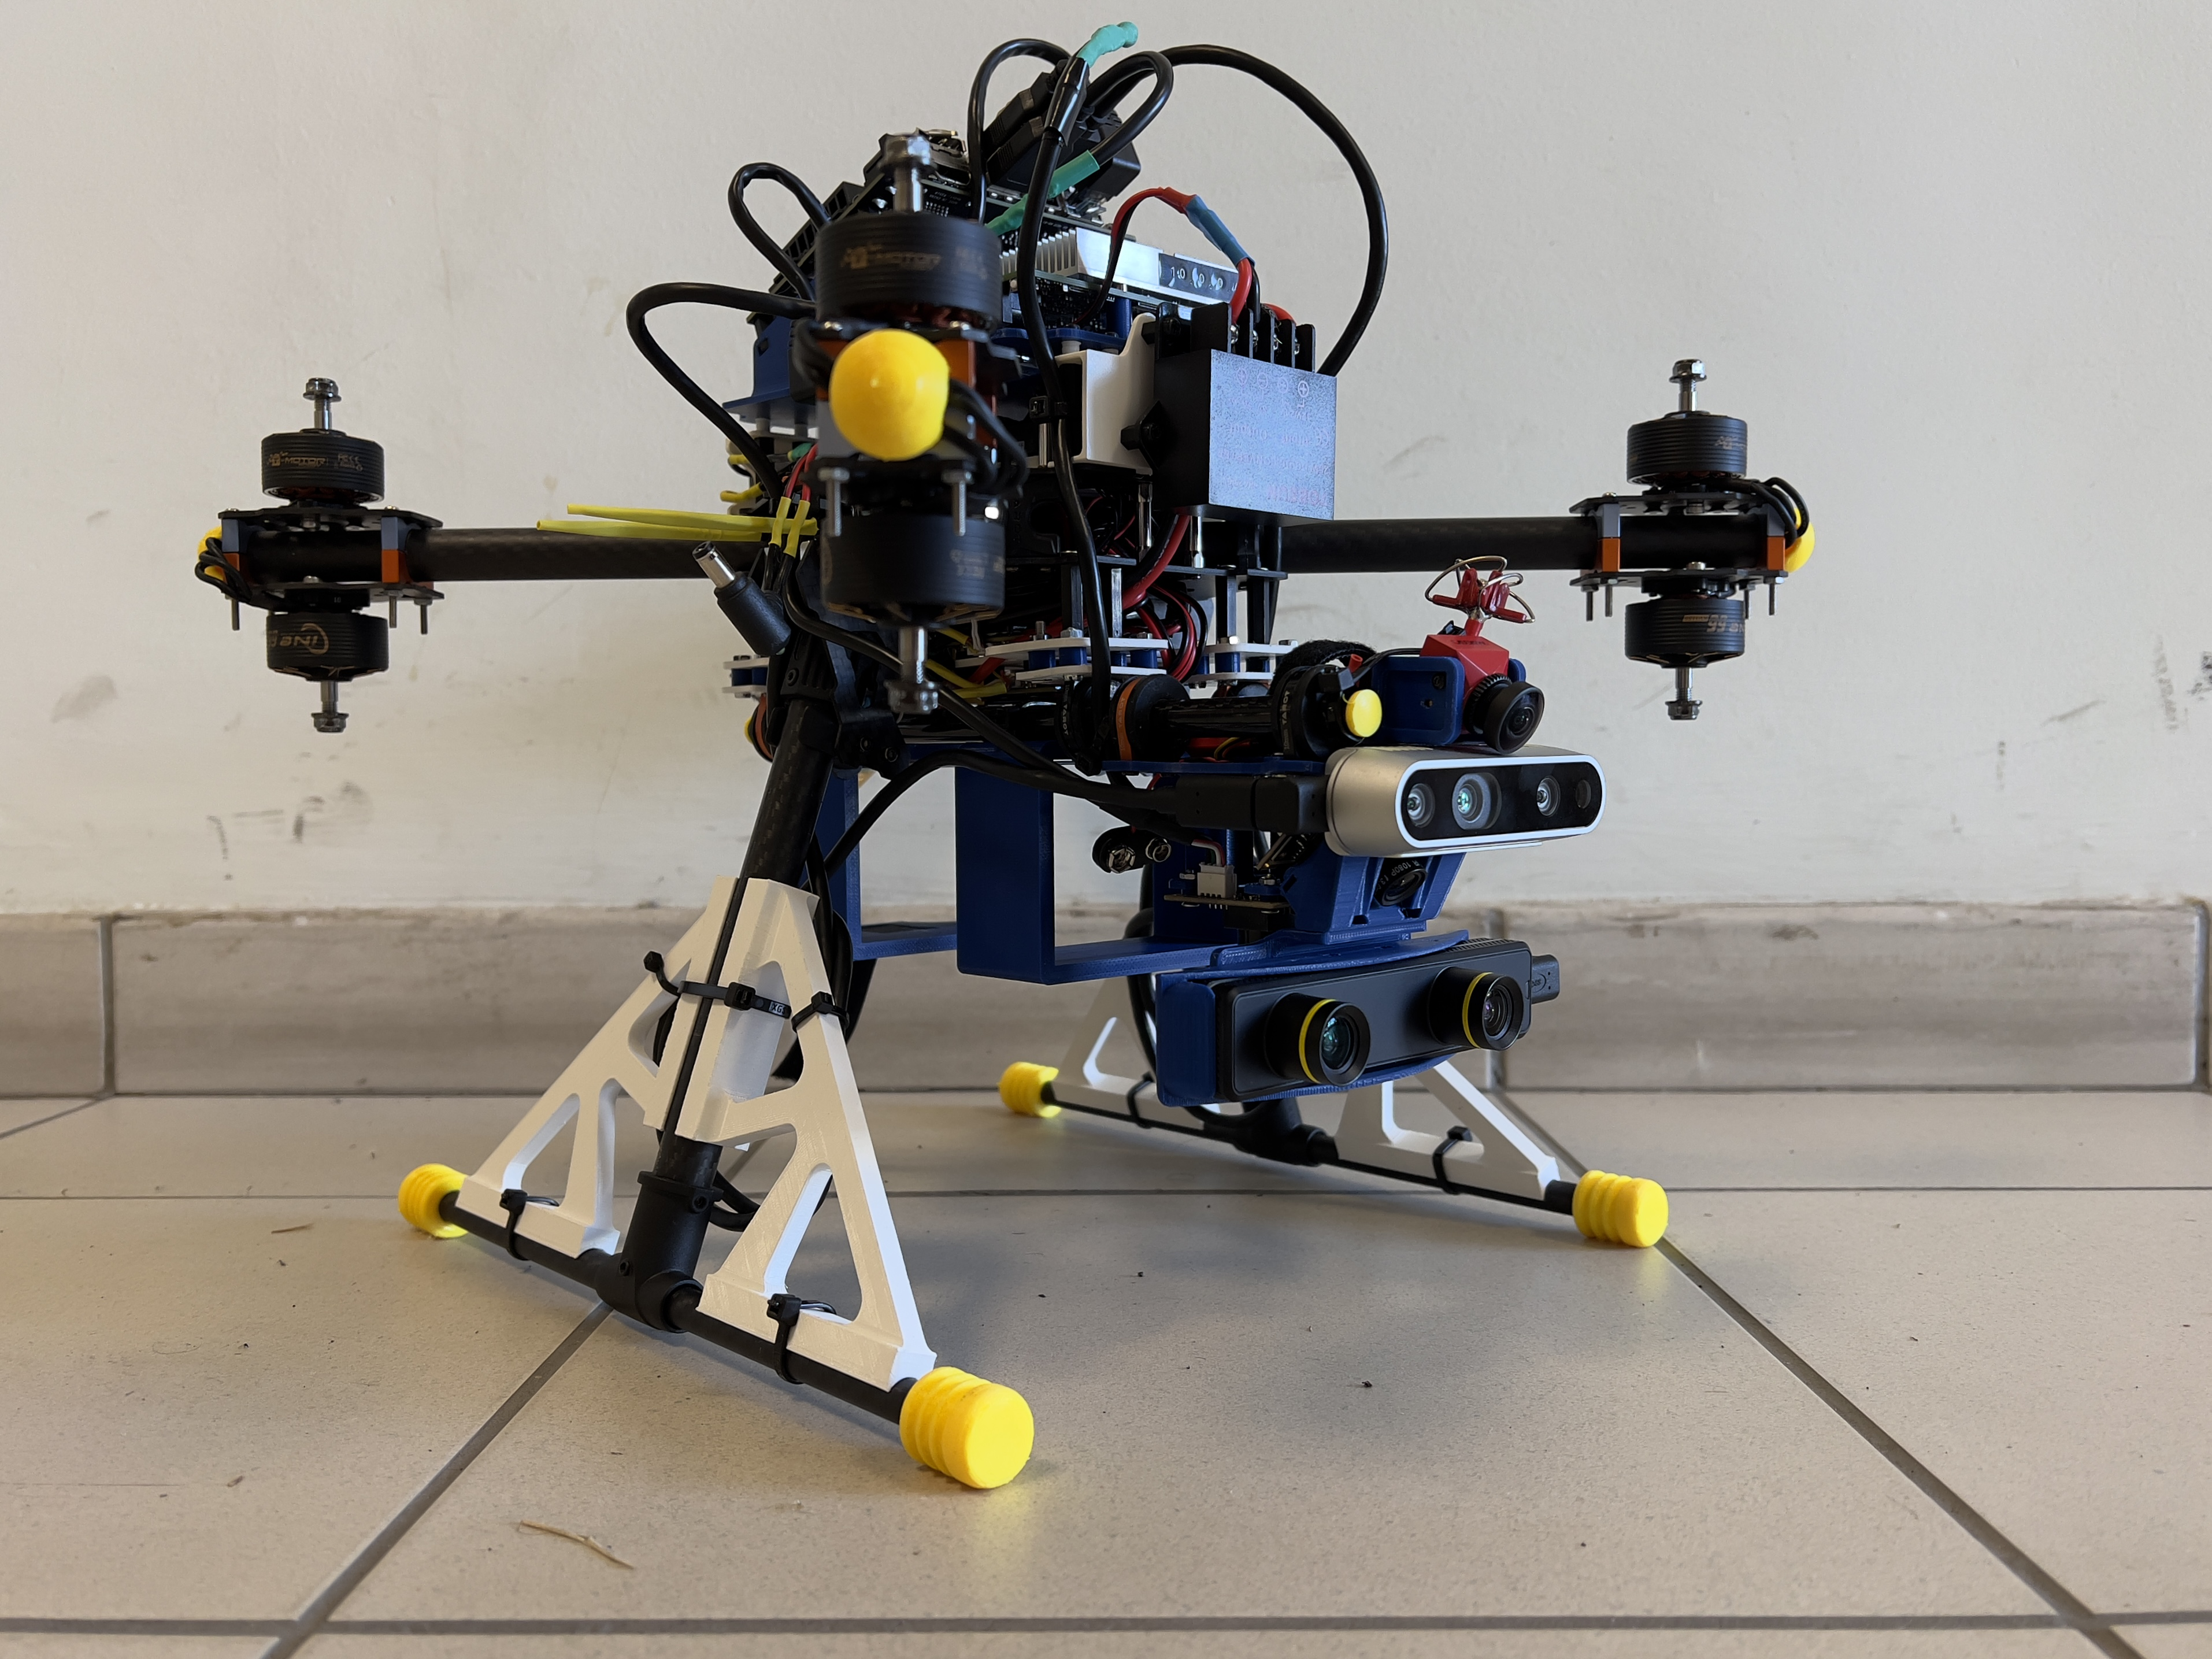
\includegraphics[width=.8\textwidth]{stanis}
			\caption{Stanis autonomous drone prototype.}
			\label{fig:stanis}
		\end{figure}
	\end{columns}
\end{frame}
\begin{frame}{The roboticist}{A new path for control engineers}
	\begin{columns}
		\column{.5\textwidth}
    \justifying
		A \textbg{roboticist} can usually:
		\begin{itemize}
			\item \textbg{design} solutions to complex problems;
			\item \textbg{develop} parts of or entire \textbg{control architectures};
			\item \textbg{deploy} and test software and hardware;
			\item make use of modern \textbg{hardware accelerators}, robotics-oriented hardware, \textbg{AI models}.
		\end{itemize}
		Industries are looking for roboticists for their \textbg{versatile skill set}.

		\column{.5\textwidth}
		\begin{figure}
			\centering
			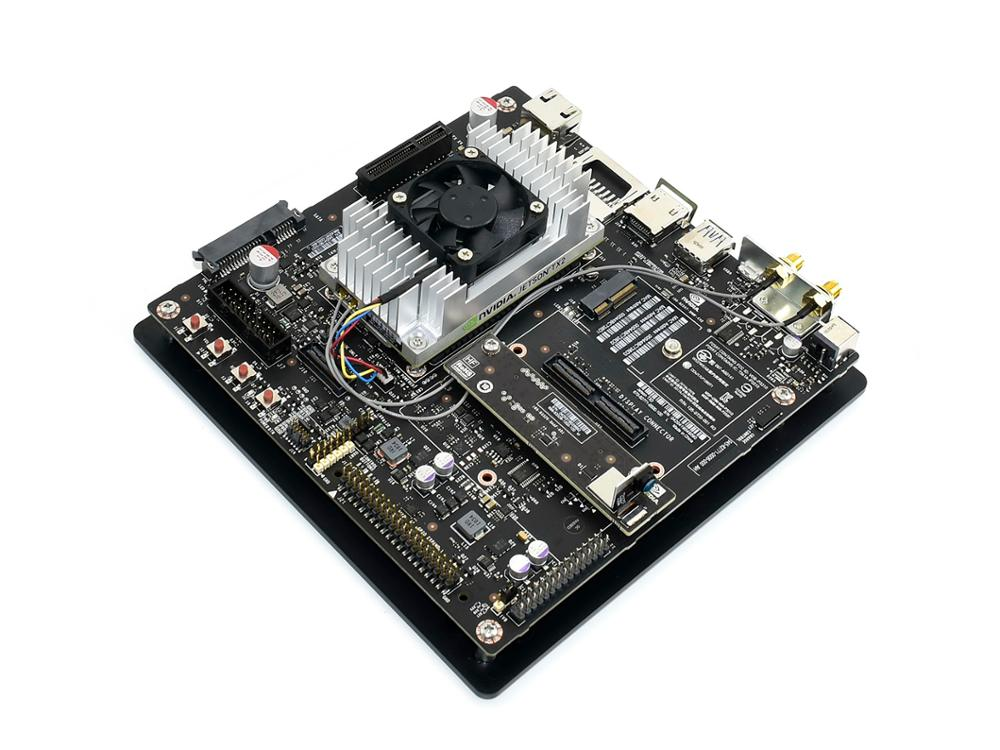
\includegraphics[width=.9\textwidth]{tx2}
			\caption{Nvidia Jetson TX2 developer kit.}
			\label{fig:tx2}
		\end{figure}
	\end{columns}
\end{frame}
